\section{QFAST Algorithm}

\subsection{Top-Down vs Bottom-Up Synthesizers}
\begin{frame}
\frametitle{Top-Down vs Bottom-Up Synthesizers}
\begin{figure}
  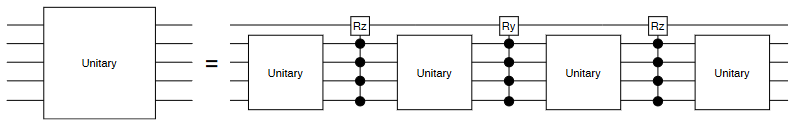
\includegraphics[width=\textwidth]{figure/top-down.png}
  \caption{Top-down synthesizers,decompose large unitaries into smaller ones while maintaining equality}
\end{figure}
% figure here
\end{frame}
\begin{frame}
  \frametitle{Top-Down vs Bottom-Up Synthesizers}
  \begin{figure}
    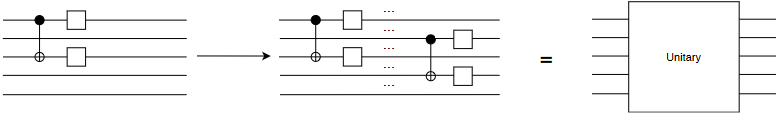
\includegraphics[width=\textwidth]{figure/bottom-up.png}
    \caption{Bottom-up synthesizers start with an empty circuit and build up to equality.}
  \end{figure}
  \begin{figure}
    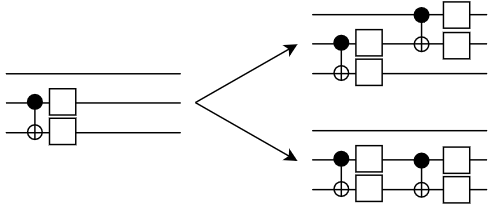
\includegraphics[width=.3\textwidth]{figure/Qsearch.png}
    \caption{QSearch uses native gates in synthesis and searches for structure in their circuit space.}
  \end{figure}
  % figure here
\end{frame}
\subsection{Introduction to QFAST Algorithm}
\begin{frame}
\frametitle{Basic idea to QFAST Algorithm}
\begin{itemize}
  \item use function to represent gates and circuits
  \item replaces expensive searches over circuit structures with numerical optimization
\end{itemize}
% work flow here
\end{frame}

\subsection{Gate Representation}
\begin{frame}
\frametitle{Gate Representation}

\begin{align}
  &F(Q, \vec{\alpha})=P_{Q}(G(\vec{\alpha}) \otimes I) P_{Q}^{T}\\
  &V(\vec{Q}, \vec{\alpha}, \vec{l})=\left(\sum_{Q \in \vec{Q}} l_{Q} \cdot P_{Q}\right)(G(\vec{\alpha}) \otimes I)\left(\sum_{Q \in \vec{Q}} l_{Q} \cdot P_{Q}^{T}\right)
\end{align}
where
\begin{align}
  G(\vec{\alpha})=e^{\mathrm{i}\left(\vec{\alpha} \cdot \sigma^{\vec{\otimes} n}\right)}
\end{align}
%  result formula
\end{frame}

\subsection{Cost Function for Optimization}
\begin{frame}
\frametitle{Cost Function for Optimization}
derive form Frobenius norm
\begin{align}
  \Delta\left(U_{C}, U_{T}\right)=1-\frac{\left|\operatorname{Tr}\left(U_{T}^{\dagger} U_{C}\right)\right|}{d}
\end{align}
% function here and how to optimize
\end{frame}
\begin{frame}
  \frametitle{work flow}
  \begin{itemize}
    \item decomposition
    \item instantiation
    \item recombination
  \end{itemize}
  \begin{figure}
    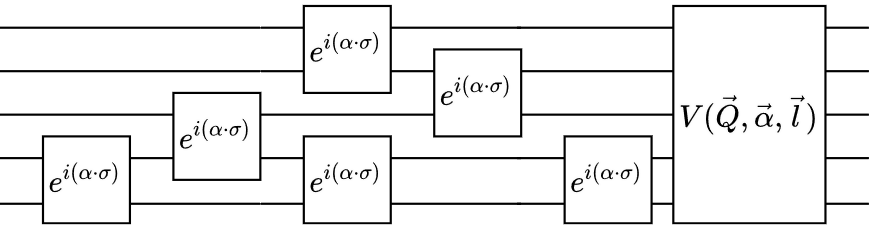
\includegraphics[width=.2\textwidth]{figure/decom.png}
  \end{figure}
\end{frame}

\subsection{Comparison with Other Algorithms}
\begin{frame}
\frametitle{Comparison with Other Algorithms}
\begin{itemize}
  \item Evaluation Metrics:
  \begin{itemize}
    \item total CNOT gate count
    \item total count of single qubit gates
    \item critical path length
    \item average gate parallelism
    \item scalability and execution time
  \end{itemize}
  \item Benchmark: Transverse Field Ising Models
  \item 3-7 qubits
\end{itemize}
% how to compare and the metrics
\end{frame}
\begin{frame}
\frametitle{Comparison results}
compare with Qiskit on average:
\begin{itemize}
  \item $10\times$ fewer CNOT gates
  \item $5.2\times$ fewer U3 gates
  \item $5.7\times$ decrease of the circuit critical
  \item $1.03\times$ better parallelism
  \item $15\times$ slower than IBM Qiskit
  \item Qiskit:$10^{-14}$,QFAST: $10^{-6}$
\end{itemize}
\end{frame}
\begin{frame}
  \frametitle{Comparison results}

  \begin{table}[]
    \begin{tabular}{l|lll}
    tfim-7-20  & Qiskit mapped & Qiskit synthesized & QFAST  \\\hline
    singal gate    & 260           & 19360              & 89     \\
    CNOT           & 240           & 18653              & 41     \\
    critical patth & 152           & 89478              & 55     \\
    pararllelism   & 3.29          & 1.03               & 2.77   \\
    time           & 0.61          & 13222.11           & 307.57
    \end{tabular}
    \caption{In terms of ALL-to-ALL synthesis results. QFAST time out when running the tfim-7-40 and tfim-7-100 benchmark examples}
    \end{table}
\end{frame}
\begin{frame}
  \frametitle{Comparison results}

  \begin{table}[]
    \begin{tabular}{l|lll}
    tfim-7-100  & Qiskit mapped & Qiskit synthesized & QFAST  \\\hline
    ssingal gate    & 1300          & 89483              & 87      \\
    CNOT           & 1200          & 58316              & 40      \\
    critical patth & 712           & 82915              & 49      \\
    pararllelism   & 3.51          & 1.78               & 2.59    \\
    time           & 6.09          & 705.01             & 8208.44
    \end{tabular}
    \caption{In terms of Linear synthesis results.}
    \end{table}
\end{frame}
\begin{frame}
